%%%%%%%%%%%%%%%%%%%%%%%%%%%%%% -*- Mode: Latex -*- %%%%%%%%%%%%%%%%%%%%%%%%%%%%
%% 04-18.tex -- Thesis Proposal for Masters
%% Author          : Takuya Yamashita
%% Created On      : Mon Sep 23 11:52:28 2002
%% Last Modified By: Takuya Yamashita
%% Last Modified On: Thu Dec  2 00:08:51 2004
%% RCS: $Id$
%%%%%%%%%%%%%%%%%%%%%%%%%%%%%%%%%%%%%%%%%%%%%%%%%%%%%%%%%%%%%%%%%%%%%%%%%%%%%%%
%%   Copyright (C) 2004 Takuya Yamashita
%%%%%%%%%%%%%%%%%%%%%%%%%%%%%%%%%%%%%%%%%%%%%%%%%%%%%%%%%%%%%%%%%%%%%%%%%%%%%%%
%%


%%\documentclass[11pt,twocolumn]{article}
\documentclass[11pt,proposal,times,thesis,actual]{uhthesis2e}
\input{/export/home/csdl/tex/psfig/psfig}
%%\usepackage{/export/home/csdl/tex/icse2003/latex8}
\usepackage{times}
\usepackage{comment}
%% A verbatim-like environment which allows font changes
%%\usepackage{alltt}
%% New LaTeX2e graphics support
\usepackage[final]{graphicx}
\usepackage{url}
%% \usepackage{rotating}
% uncomment the % away on next line to produce the final camera-ready version
% and uncomment the \thispagestyle{empty} following \maketitle
\pagestyle{empty}

\begin{document}

\title{Evaluating Automated Review Process:  \\ Jupiter incorporating with Hackystat}
\author{\protect\begin{tabular}{ccc}
Takuya Yamashita\\
\end{tabular}\\
\em Collaborative Software Development Laboratory\\
\em Department of Information and Computer Sciences\\
\em University of Hawai'i\\
\em Honolulu, HI, 96822\\
\em takuyay@hawaii.edu} \degreemonth{December} \degreeyear{2005}
\degree{Masters} \chair{Philip M. Johnson} \othermembers{}
\numberofmembers{5} \field{Computer Science} \maketitle
\thispagestyle{empty}

\input{04-18-abstract.tex}
%\input{04-18-intro.tex}
%\input{04-18-related.tex}
%\input{04-18-impl.tex}
\input{04-18-evaluation.tex}
%\input{04-18-timeline.tex}
%%\input{04-18-conclusion.tex}
\appendix
\chapter{Jupiter plug-in for Eclipse Evaluation Questionnaire}
\label{appendix:JupiterQuestionnaire}

\begin{figure}[htbp]
  \centering
  \includegraphics[width=1.0\textwidth]{figures/JupiterQuestionnaire_1.eps}
  \label{fig:JupiterQuestionnaire_1}
\end{figure}

\begin{figure}[htbp]
  \centering
  \includegraphics[width=1.0\textwidth]{figures/JupiterQuestionnaire_2.eps}
  \label{fig:JupiterQuestionnaire_2}
\end{figure}

\begin{figure}[htbp]
  \centering
  \includegraphics[width=1.0\textwidth]{figures/JupiterQuestionnaire_3.eps}
  \label{fig:JupiterQuestionnaire_3}
\end{figure}

\begin{figure}[htbp]
  \centering
  \includegraphics[width=1.0\textwidth]{figures/JupiterQuestionnaire_4.eps}
  \label{fig:JupiterQuestionnaire_4}
\end{figure}

\begin{figure}[htbp]
  \centering
  \includegraphics[width=1.0\textwidth]{figures/JupiterQuestionnaire_5.eps}
  \label{fig:JupiterQuestionnaire_5}
\end{figure}

\begin{figure}[htbp]
  \centering
  \includegraphics[width=1.0\textwidth]{figures/JupiterQuestionnaire_6.eps}
  \label{fig:JupiterQuestionnaire_6}
\end{figure}

\begin{figure}[htbp]
  \centering
  \includegraphics[width=1.0\textwidth]{figures/JupiterQuestionnaire_7.eps}
  \label{fig:JupiterQuestionnaire_7}
\end{figure}

\begin{figure}[htbp]
  \centering
  \includegraphics[width=1.0\textwidth]{figures/JupiterQuestionnaire_8.eps}
  \label{fig:JupiterQuestionnaire_8}
\end{figure}

\begin{figure}[htbp]
  \centering
  \includegraphics[width=1.0\textwidth]{figures/JupiterQuestionnaire_9.eps}
  \label{fig:JupiterQuestionnaire_9}
\end{figure}

\begin{figure}[htbp]
  \centering
  \includegraphics[width=1.0\textwidth]{figures/JupiterQuestionnaire_10.eps}
  \label{fig:JupiterQuestionnaire_10}
\end{figure}


\bibliography{/export/home/csdl/bib/tdd,/export/home/csdl/bib/csdl-trs}
\bibliographystyle{plain}

\end{document}
